\section{Tryb przetwarzania danych}

\paragraph{Przetwarzanie lokalne}
Pierwszy zaimplementowany system wykonywał całe przetwarzanie zebranych danych~na~mapy cieplne~na~telefonie użytkownika. Gotowe obrazki były wysyłane~i~składowane~w~chmurze. To~podejście zostało wybrane~ze~względu~na~swoją prostotę, jednak~po~pierwszych testach okazało się nieodpowiednie. Podczas jednej wizyty~w~aplikacji  użytkownik odwiedza średnio parę stron,~na~każdej wykonując parę (często~tylko~jedną) interakcję. Z~każdej wizyty tworzone było~więc~parę prawie pustych map cieplnych. Podczas pierwszych testów stało się jasne,~że~to~podejście charakteryzuje się stanowczo zbyt dużym rozdrobnieniem danych. Przeprowadzenie ewaluacji używając przetwarzania lokalnego, spowodowałoby powstanie setek mało interesujących obrazków, których~nie~sposób byłoby przeanalizować.

\paragraph{Przetwarzanie zdalne}
Rozwiązaniem tego problemu było oddzielenie części przetwarzającej dane~na~mapy cieplne (procesora graficznego)~do~osobnego programu tworząc aktualną architekturę narzędzia zamieszczoną~na~rysunku \ref{fig:round_spot_diagram}. Zamiast gotowych obrazków~do~chmury przesyłane~są~zserializowane, surowe dane~o~ekranie~i~działaniach użytkownika. Dzięki temu wszystkie interakcje~na~danym ekranie zebrane podczas ewaluacji mogą być umieszczone~na~pojedynczej mapie cieplnej. Takie podejście daje też dużo większą swobodę~i~kontrolę~nad~postacią danych wyjściowych. Mogą być one dowolnie grupowane~i~dzielone~w~celu uzyskania jak największej ilości informacji~i~wniosków.

\section{Tworzenie map przewijanych}
Największa trudność napotkana podczas implementacji dotyczyła zbierania danych~z~obszarów przewijanych, które~nie~mieszczą się~w~całości~na~ekranie aplikacji. Detektor może zostać umieszczony~w~drzewie elementów interfejsu~na~dwa sposoby (zilustrowane~na~rysunku \ref{fig:rs_scroll_diagram}), jako rodzic obszaru przewijanego~lub~jego dziecko. W~zależności~od~tego jego pole widzenia~i~rozmiar będą się różniły. Jeśli jest dzieckiem (znajduje się~w~środku obszaru)~ma~dostęp~do~całej jego zawartości, nawet tej aktualnie niewyświetlonej. W~przeciwnym wypadku (będąc rodzicem obszaru) znajduje się~naokoło niego~i~``widzi'' jedynie aktualnie wyświetloną~na~ekranie zawartość.

\img{\chapterPath/scroll-diagram.png}{Możliwości zbierania danych~o~obszarach przewijanych}{rs_scroll_diagram}{.6}

\subsection{Pierwsze podejście}
Pierwszym wybranym podczas implementacji podejściem było umieszczenie detektora~w~środku obszaru przewijanego. Dzięki dostępowi~do~całej zawartości~w~każdym momencie stworzenie jej obrazu~do~późniejszego użycia~w~mapie cieplnej było~tak~samo łatwe jak~w~przypadku nieprzewijanych obszarów. Podczas testów okazało się~że~to~podejście, chociaż proste,~ma~poważne wady.

\paragraph{Zdarzenia~we~Flutterze}
Dotknięcia ekranu nazywane zdarzeniami \ang{events},~są~zaimplementowane~we~Flutterze podobnie jak~w~standardzie DOM używanym~przez~przeglądarki. Po~rejestracji~przez~urządzenie zdarzenie jest przekazywane~od~korzenia drzewa elementów interfejsu (czyli całej strony)~w~głąb~do~kolejnych dzieci zajmujących obszar zawierający współrzędne dotknięcia. Ten proces jest rekurencyjnie powtarzany~do~czasu gdy zdarzenie zostanie ``wykorzystane''~lub~przekazane~do~liścia drzewa. Wykorzystanie oznacza podjęcie akcji takiej jak naciśnięcie przycisku.

Jedną~z~możliwych akcji jest gest przewijania obszaru ekranu. W~wybranym podejściu,~w~którym detektory~są~dziećmi elementów przewijanych,~nie~otrzymają one informacji~o~zdarzeniach przewijania, gdyż zostaną one zatrzymywane~przez~ich rodziców. Ta~wada była~nie~do~zaakceptowania~z~powodu straty dużej ilości potencjalnie interesujących informacji~o~działaniach użytkownika.

\subsection{Zastosowane rozwiązanie}
Drugim dostępnym podejściem~do~tworzenia tła map przewijanych według rysunku \ref{fig:rs_scroll_diagram} jest umieszczenie detektorów jako rodziców obszarów przewijanych. Zastosowanie~go~rozwiązało problem utraty informacji~o~przewijaniu ekranu, jako~że~każde zdarzenie przechodziło~przez~detektor~na~drodze~do~jego dziecka. Rozwiązanie~to~jest też bardziej ogólne~i~w~przyszłości może pozwolić~na~znaczne uproszczenie użycia narzędzia~przez~twórców aplikacji, opisane~w~sekcji \ref{sec:auto_instrumentation}. 

Z tym podejściem wiąże się jednak duża komplikacja procesu uzyskiwania obrazu tła przewijanego obszaru. Ponieważ detektor~ma~dostęp~tylko~i~wyłącznie~do~jego aktualnie wyświetlanej części, podczas przewijania muszą być stale zapisywane kolejne fragmenty ekranu. Te~częściowe obrazki wraz~z~informacją~o~ich przesunięciu względem górnej krawędzi obszaru~są~następnie sklejane~w~jedno spójne tło wykorzystywane przy tworzeniu przewijanych map cieplnych.

Implementacja tego mechanizmu stanowiła wyzwanie~na~wielu płaszczyznach. Rozwiązanie musiało wspierać zarówno przewijanie~w~pionie jak~i~w~poziomie. Jednym~z~wymagań było stworzenie nieprzerwanego tła~bez~względu~na~szybkość przewijania ekranu. Aby osiągnąć ten efekt, moment zapisania kolejnego obrazu tła został uzależniony~od~części widocznego obszaru, która została przewinięta~od~momentu stworzenia poprzedniego obrazu. Ponieważ aktualne przesunięcie ekranu jest udostępniane~przez~inny komponent platformy Flutter niż wyświetlany obraz,~te~dwie informacje musiały zostać zsynchronizowane, aby uniknąć przesunięć~w~złączonym tle. Szybkie przewijanie ekranu powodowało też wyścigi związane~z~nadpisywaniem informacji. Problem został rozwiązany poprzez stworzenie kolejki asynchronicznie przetwarzającej zapisane fragmenty tła~i~łączące~je~w~całość.

\section{Łączenie danych~z~wielu urządzeń}
Głównym wyzwaniem napotkanym podczas implementacji procesora danych okazał się wpływ różnic~w~wielkości ekranów urządzeń,~z~których korzystają użytkownicy~na~wzajemne pozycje ich interakcji. W~założeniu, aby sprowadzić koordynaty dotknięć ekranów~o~różnych wielkościach~do~wspólnej przestrzeni, wystarczy~je~podzielić~przez~rozmiar ekranu,~z~którego pochodzą. W~praktyce, jak pokazano~na~rysunku \ref{fig:screen_sizes}, nawet~po~wykonaniu tej transformacji grupy punktów cieplnych~na~mapach~nie~zawsze dokładnie pasują~do~znajdujących się~pod~nimi elementów interfejsu. 

\subsection{Piksele logiczne~i~fizyczne}
Jednym~z~powodów jest specyfika jednostki,~w~której platforma podaje pozycje interakcji. Flutter używa~do~tego celu~tak~zwanych pikseli logicznych \ang{logical pixels} \cite{Logic_pixels}, znanych też~pod~nazwą pikseli niezależnych~od~rozdzielczości \ang{density/resolution/device-independent pixels - DP}. Podczas gdy piksele fizyczne~są~punktami świetlnymi~w~ekranie urządzenia,~na~którym mogą być umieszczone~z~różną gęstością, piksele logiczne mają zawsze reprezentować ten sam rozmiar wizualny~bez~względu~na~rozdzielczość ekranu. Według autorów platformy~na~jeden centymetr ekranu przypada około 38 pikseli logicznych. Użycie takiej jednostki przy rysowaniu interfejsu znacznie upraszcza skalowanie jego elementów~do~naturalnych dla użytkownika rozmiarów.

Z~powodu późnego wykrycia implikacji faktu reprezentacji współrzędnych~w~jednostkach pikseli logicznych przelicznik~na~piksele fizyczne, który może być różny dla każdego urządzenia,~nie~był zapisywany podczas przeprowadzania ewaluacji. Zamiast niego~do~przeskalowania pozycji interakcji musiał zostać użyty rozmiar ekranu~w~pikselach fizycznych odczytywany jako rozmiar dołączonych obrazów tła. Różnice pomiędzy wartościami obu jednostek przyczyniły się~do~przesunięcia pozycji interakcji względem niektórych obrazów tła.

\subsection{Wpływ rozmiaru ekranu~na~jego zawartość}
Drugim~ze~zidentyfikowanych powodów widocznych przesunięć jest wpływ rozmiaru ekranu~na~sposób rysowania elementów interfejsu~przez~platformę. Wraz~ze~zwiększaniem się ekranu tekst staje się coraz mniejszy~a~odstępy~i~marginesy rosną,~co~jest widoczne~na~rysunku \ref{fig:screen_sizes}. Ekran pokazany~po~prawej stronie jest większy~od~tego~po~lewej. Różnice~w~wielkości elementów spowodowane wielkością ekranu mogą wpływać~na~zmianę ich wzajemnych odległości,~co~w~efekcie prowadzi~do~niejednoznacznej reprezentacji punktów~w~przestrzeni ekranu~i~nieprawidłowego ułożenia części interakcji~na~wynikowych mapach cieplnych.

\bigskip
\begin{figure}[H]
\centering
\begin{minipage}{.36\textwidth}
	\centering
	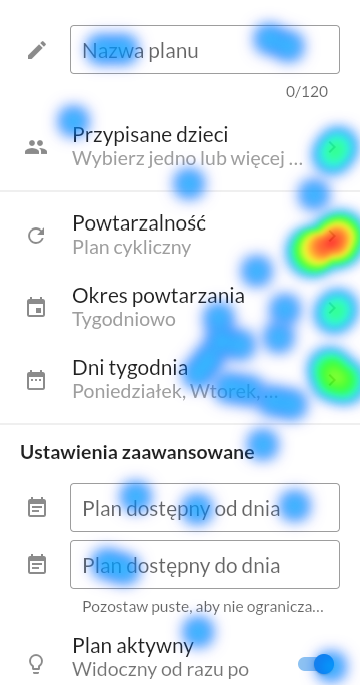
\includegraphics[width=.9\linewidth]{\chapterPath/small-screen.png}
\end{minipage}
\begin{minipage}{.4\textwidth}
	\centering
	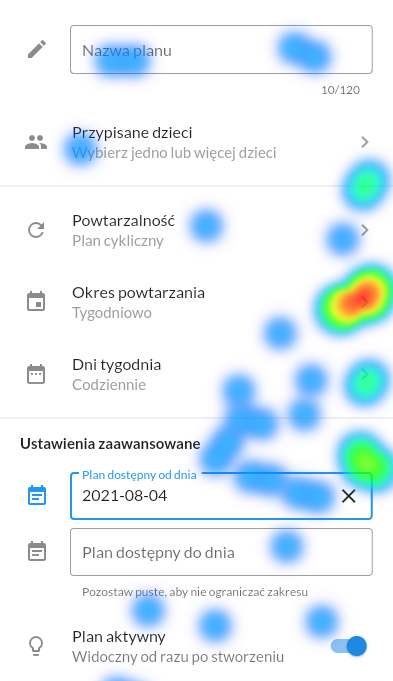
\includegraphics[width=.9\linewidth]{\chapterPath/big-screen.png}
\end{minipage}
\bigskip
\caption{Wpływ różnic~w~wielkościach ekranów}
\label{fig:screen_sizes}
\end{figure}
